\documentclass[a4paper, 11pt]{scrreprt}
\usepackage[utf8]{inputenc}
\usepackage[T1]{fontenc}
\usepackage{lmodern}
\usepackage{amsmath,amssymb,amstext,amsfonts,mathrsfs, amsthm}
\usepackage{graphicx}
\usepackage{color}

\usepackage{marginnote}

\pagestyle{headings}

\newtheorem{defi}{Definition}[section]
\newtheorem{prop}[defi]{Proposition}
\newtheorem{theorem}[defi]{Theorem}
\newtheorem{coro}[defi]{Corollary}
\newtheorem{lemma}[defi]{Lemma}

\newcommand{\RR}{\mathbb{R}}
\newcommand{\EE}{\mathbb{E}}
\newcommand{\ZZ}{\mathbb{Z}}
\newcommand{\NN}{\mathbb{N}}
\newcommand{\FF}{\mathcal{F}}

\newcommand{\student}[1]{\marginnote{{\normalfont\bf #1}}}

\title{Abschlussarbeit Fallstudien der math. Modellbildung}
\author{Manuela Lambacher, Dominik Otto, Andreas Wiedemann}
\date{\today}

\begin{document}
\parindent 0pt
\maketitle
\tableofcontents

\chapter*{Introduction}
\begin{quotation}
When you can measure what you are talking about and express it in numbers, you know something about it – Lord W. T. Kelvin
\end{quotation}

Digitalization of analog signals plays an essential role in our technology-driven society. Even simple things of our daily life, like making a phone call, are not possible without digitalizing analog signals, for example our voice. \\
\newline
Analog digital converters (short: ADC) are the interface between human and machine. Thousands of research papers have been published on the solution of this problem, bringing together mathematicians, physicists and engineers. \\
Fourier analysis provides a powerful tool for handling the task by transforming a signal from the time domain into the frequency domain. The conversion provides several advantages. Processing and Transmission of the transform is more efficient and reliable. Moreover not only the reconstruction of it is more accurate, but also it can be stored more compactly.

Often the output signal has to be analog, requiring a digital analog converter (DAC). This implies the necessity of precisely reconstructing the signal. 
Considering the special case of bandlimited \(L^2\) functions, Shannn and Whittaker were able to find a method to reconstruct functions from  sequences of real numbers. \\
\newline
%Whereas digitalizing can be done rather  straightforward by sampling, the real art is regaining the original signal from these samples or assessing the information lost in the sampling process.\\
In the following, we'd like to try to give a small survey of the Whittaker-Shannon interpolation formula, which is of high importance in communication theory. Further on we will describe its applications in real-life but also its limitations, keeping in mind the relationship of Fourier transform and the Heisenberg uncertainty principle.



\chapter{Whittaker-Shannon Interpolation formula}


\section{Preliminary notes and Sampling}
\begin{defi}[Fourier transform]
The Fourier transform \(\FF(f)\) of a d-dimensional, integrable function \(f:\RR^d \to \RR\) is given by
	\begin{equation}
		\FF f(w)=\int_{\RR^d} f(x)e^{-2\pi iwx}\,\mathrm{d}x
	\end{equation}

\end{defi}
So, the Fourier transform converts a time domain function into a frequency domain function. For example, the Fourier transform of an audio signal identifies the frequency spectrum as peaks in the frequency domain.\\
If \(\FF f\in L^1(\RR^d)\), then we can define the inverse Fourier transform:
\begin{defi}[Inverse Fourier transform]
\begin{equation}
	f(x) = \int_{\RR^d} \FF f(w) e^{2\pi iwx}\,\mathrm{d}w
\end{equation}
\end{defi}

\begin{defi}[bandlimited function]
	For \(Q = \prod_{i=1}^d \omega_i[-1/2, 1/2),\ \omega\in\RR^d\), we define
	\begin{equation}
		L_Q^2(\RR^d) = \{f\in L^2(\RR^d):\ supp(\FF f) \subset Q\}
	\end{equation}
	If \(f\in L_Q^2(\RR^d)\), then it is called \(\omega\)-bandlimited.
\end{defi}

\begin{lemma}[Bessel's inequality]
Let X be a Hilbert space, $S \subset X$ an orthonormal system. Then one has
\[\sum_{e \in S} |\langle x, e \rangle |^2 \leq \Vert x \Vert ^2\]
%Let X be a separable Hilbert space with $\dim(X) = \infty$ and $\{e_k:k \in \ZZ^d\}$ an orthonormal system. Then it is equivalent:
%\begin{itemize}
%\item[i)] $\{e_k:k \in \ZZ^d\}$ is an orthonormal basis
%\item[ii)] For all $x \in X$ Parseval's identity holds
%\[\Vert x \Vert^2 = \sum_{k\in \ZZ^d} |\langle x, e_k \rangle|^2\]
%\end{itemize}
\end{lemma}


\subsection{Sampling}
To convert a continuous function \(f\) into a sequence of discrete values is called sampling. In a mathematical way, sampling can be described as a multiplication of \(f\) with a dirac-comb 
\[s(t,\Delta T) = \sum_{n\in\ZZ} \delta(t-n\Delta T), \]
where \(\Delta T\) is the sampling intervall and \(\delta\) is the Dirac-function.\\
The sampled function \(\tilde{f}\) of our original \(f\) is denoted by
\begin{equation}
	\tilde{f} (t) = s(t,\Delta T) f(t) = \sum_{n\in\ZZ} f(t)\delta(t-n\Delta T)
\end{equation}
\begin{figure}[htpb]
	\centering
	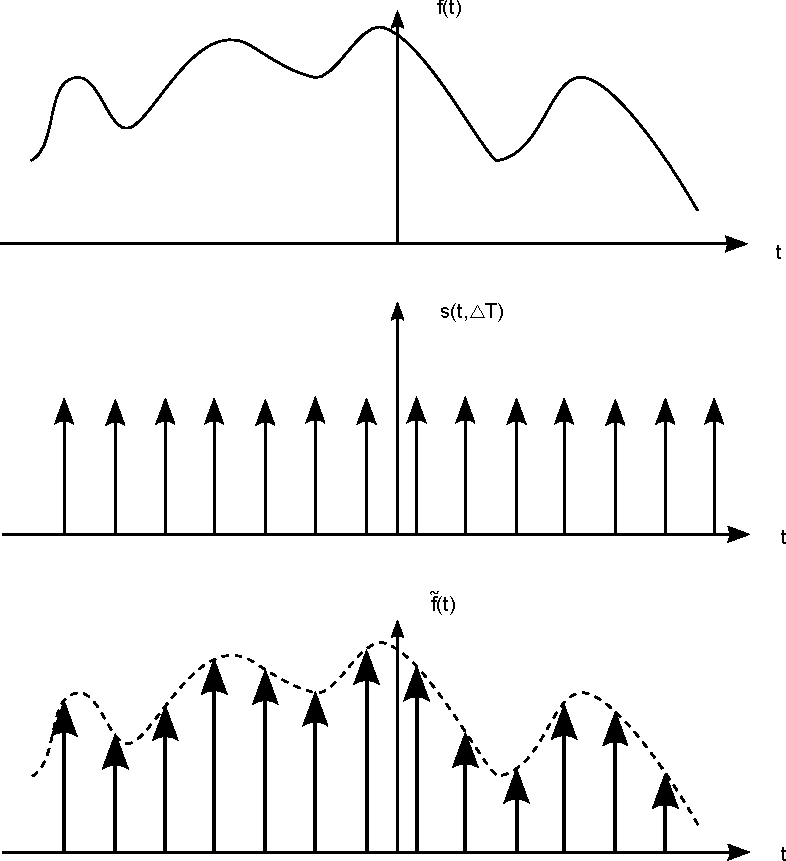
\includegraphics[width=0.55\textwidth]{Sampling-Visualisierung.pdf}
	\caption{(a) continuous function \(f\), (b) the dirac-comb, (c) sampled function as product of (a) and (b)}
\end{figure}
(see \cite{marks02})\\

The following theorem will be essential for our further work:
\begin{theorem}[perturbed sampling in \(L^2\)]
\label{th:perturbed sampling}
Let \(Q = \prod_{i=1}^d \omega_i[-1/2, 1/2)\) and \\
 \({f\in C(\RR^d)\cap L^2(\RR^d)}\) such that \(f_{|\tau\ZZ^d} \in l^2\). We write \(f=\eta + \epsilon\), where \(\FF\eta = \FF f\) on \(Q\). Then it holds
\begin{equation}
	f(x) = \sum_{k\in\ZZ^d} (f^c(\tau k)-\epsilon^c(\tau k))\prod _{i=1}^d sinc(\tau_i^{-1}x_i-k_i)+\epsilon(x), \qquad \text{in } L^2(\RR^d),
\end{equation}
where \(sinc(x) = \frac{sin(\pi x)}{\pi x}\).
\end{theorem}

\newpage
\section{The Whittaker-Shannon Interpolation formula}

\begin{theorem}[Interpolation formula]
\label{th:interpolation}
If \(f \in L^2(\RR^d)\) is a \(\omega\)-bandlimited function, there exists a \(\tau_0 > 0\) such that for all \(\tau \in \left(0,\tau_0\right]\)
\begin{equation}
	f(x) = \sum_{k \in \ZZ^d} f^c(\tau k) \prod_{i=1}^d sinc\left(\tau_i^{-1} x_i -k_i\right).
\end{equation}
\end{theorem}
In other words, every bandlimited \(L^2\) function can be perfectly reconstructed from its infinitely but countable many samples, if the sampling rate is high enough!\\

\begin{proof}[Proof]
We will prove the assertion by using theorem \ref{th:perturbed sampling}.\\ Let $f \in L^2(\RR^d)$ be a $\omega$-bandlimited function and set $\tau_0 := \frac{1}{\omega} = \left(\frac{1}{\omega_0}, \ldots, \frac{1}{\omega_d}\right)$ and $\epsilon := 0$. Besides choose $\tau \in (0,\tau_0]$ arbitrarily and define $T := \prod_{i=1}^d \left[-\frac{1}{2\tau_i} ,\frac{1}{2\tau_i}\right]$ and $Q := \prod_{i=1}^d \left[-\frac{1}{2}\omega_i ,\frac{1}{2}\omega_i\right]$.
\begin{itemize}
\item[i)] Since \(\FF(f)\) has a compact support and is continuous, $\FF(f)$ takes a maximal value $\Vert \FF(f) \Vert_\infty$. This leads to $\int_{\RR^d}| \FF f(w)|dw = \int_Q| \FF f(w)| dw \leq \Vert \FF(f) \Vert_\infty \mathscr{L}(Q) < \infty$. Therefore $\FF(f) \in L^1(\RR^d)$ and the fourier transform is reversible.
	 \[f(x) = \FF^{-1}(\FF(f))(x) = \int_{\RR^d}\FF(f)(\hat{x}) e^{2 \pi i (\hat{x},x)} d\hat{x}\]
	 Hence you can differentiate $f$.
	 \[df(x) = \left(\int_{\RR^d} \FF(f)(\hat{x}) e^{2 \pi i (\hat{x},x)} 2 \pi i \hat{x}_1 d\hat{x}, \ldots, \int_{\RR^d} \FF(f)(\hat{x}) e^{2 \pi i f t} 2 \pi i \hat{x}_d d\hat{x} \right)\]
	 You can easily see now that \(f \in C^\infty(\RR^d)\), thus $f \in C(\RR^d) \cap L^2(\RR^d)$.
\item[ii)] Now we want to show that $\{\det(\tau)^{d/2}\ e^{2 \pi i (w,k \tau)}\}_{k \in \ZZ^d}$ is an orthonormal system of $L^2(T)$.
\begin{align*}
\forall k,l \in \ZZ^d: \langle e_k(w), e_l(w) \rangle 
&= \det(\tau) \int_{T} e^{2 \pi i (\langle w,k \tau \rangle- \langle w,l \tau \rangle )}dw
= \det(\tau) \int_{T} e^{2 \pi i \langle w,(k-l) \tau \rangle}dw \\
&= \int_{-\frac{1}{2\tau_1}}^{\frac{1}{2\tau_1}} \cdots \int_{-\frac{1}{2\tau_d}}^{\frac{1}{2\tau_d}} \prod_{j=1}^d \tau_j e^{2 \pi i w_j (k_j-l_j) \tau_j}dw_1 \ldots dw_j \\
&= \prod_{j=1}^d \int_{-\frac{1}{2\tau_j}}^{\frac{1}{2\tau_j}} \tau_j e^{2 \pi i w_j (k_j-l_j) \tau_j}dw_j
\end{align*}

If $k \neq l$, then there is a $j \in \{1,\ldots,d\}$ such that $k_j \neq l_j$. With regard to the integral, it means:

\begin{align*}
\int_{-\frac{1}{2\tau_j}}^{\frac{1}{2\tau_j}} \tau_j e^{2 \pi i w_j (k_j-l_j) \tau_j}dw_j
&= \left[ \frac{1}{2 \pi i (k_j - l_j)} e^{2 \pi i w_j (k_j-l_j) \tau_j} \right]_{w_j = -\frac{1}{2 \tau_j}}^{\frac{1}{2 \tau_j}} \\
&= \frac{1}{2 \pi i (k_j-l_j)} \left( e^{\pi i (k_j-l_j)} - e^{-\pi i (k_j-l_j)} \right) = 0
\end{align*}

In case $k = l$ we can conclude:
\[\prod_{j=1}^d \int_{-\frac{1}{2\tau_j}}^{\frac{1}{2\tau_j}} \tau_j e^{2 \pi i w_j (k_j-l_j) \tau_j}dw_j
= \prod_{j=1}^d \tau_j \left(\frac{1}{2\tau_j}+\frac{1}{2\tau_j}\right) = 1\]

Consequently $\{\det(\tau)^{d/2}\ e^{2 \pi i (w,k \tau)}\}_{k \in \ZZ^d}$ is an orthonormal system of $L^2(T)$. (It is even an orthonormal basis.)

That's why one has Bessel's inequality.
\begin{align*}
\sum_{k \in \ZZ^d} |f(k \tau)|^2
&= \sum_{k \in \ZZ^d} | \int_{\RR^d} \FF f(w) e^{2 \pi i \langle w,k \tau \rangle}dw|^2 \\
&= \sum_{k \in \ZZ^d} | \left\langle \FF f(w), e^{2 \pi i \langle w,k \tau \rangle}\right\rangle |^2
\leq (\det(\tau))^{-d} \Vert \FF f \Vert_{L^2(T)}^2 < \infty
\end{align*}
So the condition $f_{|\tau\ZZ^d} \in l^2$ is fulfilled.

\end{itemize}

So theorem \ref{th:perturbed sampling} is applicable and we can conclude:
\begin{align*}
f(x) &= \sum_{k\in\ZZ^d} (f^c(\tau k)-\epsilon^c(\tau k))\prod _{i=1}^d sinc(\tau_i^{-1}x_i-k_i)+\epsilon(x) \\
&= \sum_{k \in \ZZ^d} f^c(\tau k) \prod_{i=1}^d sinc\left(\tau_i^{-1} x_i -k_i\right)  
\end{align*}

\end{proof}
\begin{figure}[htpb]
	\centering
	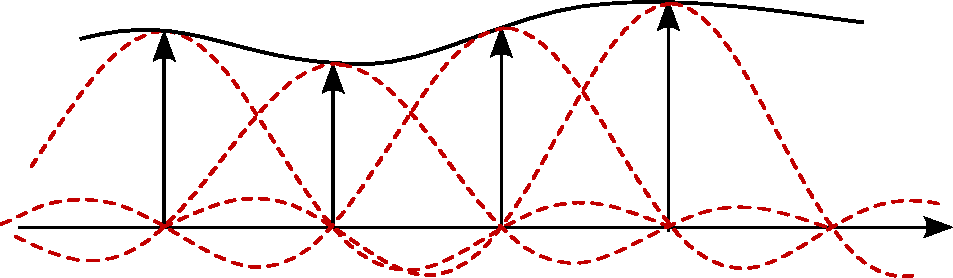
\includegraphics[width=0.80 \textwidth]{Rekonstruktion-Visualisierung.pdf}
	\caption{Visualisation of the interpolation formula for \(d=1\): the original signal (black line) is reconstructed by weighted and shifted sinc-functions}
\end{figure}


\newpage
\section{Meaning, real-life applications and limitations}

\subsection{Meaning}

Now we know, that a band-limited \(L^2\) function can be perfectly reconstructed with \(\tau_0\) small enough. Indeed, it is possible to determine \(\tau_0\) more precisely:
\begin{theorem}[Shannon-Nyquist sampling theorem]
\label{th:sampling}
Let \(f\in L^2_Q(\RR^d)\), \(\lambda_{max}\) the highest frequency of \(f\), \(\frac{1}{\tau}\in \RR^d\) the sampling rate. If \(\frac{1}{\tau_0} \geq 2\cdot \lambda_{max}\), \(f\) can be reconstructed from its samples for all \(\tau \leq \tau_0\).\\
\(\frac 1 2 \frac{1}{\tau_0}\) is called the Nyquist-rate or Nyquist-frequency.
\end{theorem} 
\begin{proof}
See \cite{shannon01}.
\end{proof}
(den Beweis abzuschreiben waere gar zu klaegliche Platzverbraucherei oder? ;))\\
\textbf{Remark:}
\begin{itemize}
\item The Whittaker-Shannon interpolation formula (Theorem  \ref{th:interpolation}) and the Shannon-Nyquist sampling theorem (Theorem \ref{th:sampling}) are often combined as the "Shannon-Nyquist-Whittaker sampling theorem".
\item According to \cite{landau04} the sampling theorem can be interpreted in another way,  apart from the reconstruction of a sampled signal, which we will not discuss further, but like to mention: \\
A sequence \(\{x_n\}\in l^2\) can be transmitted with rate \(2W\) (=Nyquist-rate) per second over an ideal channel of bandwith \(W Hz\), where \(\{x_n\}\) represents the samples of a bandlimited \(L^2\) signal.

\end{itemize}
The problem about Theorem  \ref{th:interpolation} and Theorem \ref{th:sampling} is that they are highly theoretical and could only be used in an ideal environment. The perfect reconstruction of a signal is not possible, since we would need infinitely many sampling points. But we can interpolate the original signal with arbitrary precision, if we just add enough sampling points. This is true because \(f(t)\to 0\) for \(t\to\pm\infty\), since \(f\in L^2\). So there is an interval \(I\) outside of which the samples are negligible small. If we sample over \(I\) at the Nyquist rate (or higher), the signal is characterized well enough, for \(I\) sufficiently large. (see \cite{marks02})\\
Even worse, Theorem  \ref{th:interpolation} and Theorem \ref{th:sampling} cannot be used for discontinuous signals or periodical signals, which are not in \(L^2\). As we will see later (see section \ref{se:uncertainty} Uncertainty principle), they even can't be used for finite signals, because finite signals are not bandlimited. \\


In order to reduce the amount of data, you might try to sample a signal with a frequency below the Nyquist rate (undersampling). However, a possible risk is to receive a deficient reconstruction of the digitalized function. We want to illustrate this by following example.

Examine $f:\RR \rightarrow \RR, f(x) = \cos(x)$ and the sample rate $\tau = 2 \pi$. For the sample function you obtain:
\[g(x) = \sum_{k \in \ZZ} f(2\pi k) sinc(\frac{x}{2 \pi}- k) = \sum_{k \in \ZZ} sinc(\frac{x}{2 \pi}- k)\]

\begin{figure}[htpb]
\centering
	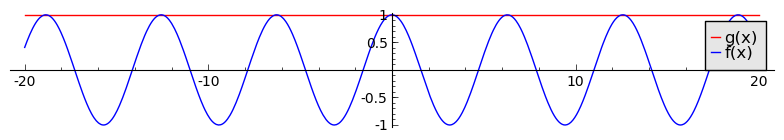
\includegraphics[height=0.2\textwidth]{SampleFunction.png}
\end{figure}


\subsection{Uncertainty Principle}
\label{se:uncertainty}
\begin{theorem}[Uncertainty principle]
Let \(g\in L^2(\RR) \) and \(a,b \in\RR\) two arbitrary scalars. Then
\begin{equation}
\label{eq:uncertainty}
\left(\int_{\RR} (x-a)^2|g(x)|^2 \,\mathrm{d}x\right)^{1/2}\left(\int_{\RR}(\omega-b)^2|\FF g(\omega)|^2\,\mathrm{d}\omega\right)^{1/2} \geq \frac{||g||_2^2}{4\pi}
\end{equation}
\end{theorem}
Which means, that an analyzing function (window) cannot be arbitrarily concentrated in the time- and frequency-domain at the same time. So a signal with compact support is not bandlimited, whereas a bandlimited signal can't be compactly supported (in particular not finite).\\
\begin{figure}[htpb]
	\centering
	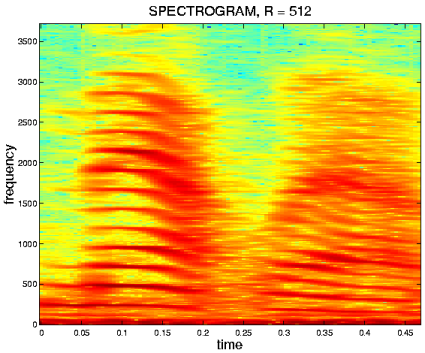
\includegraphics[height=0.40\textwidth]{Narrow-band-spectrogram.png}
	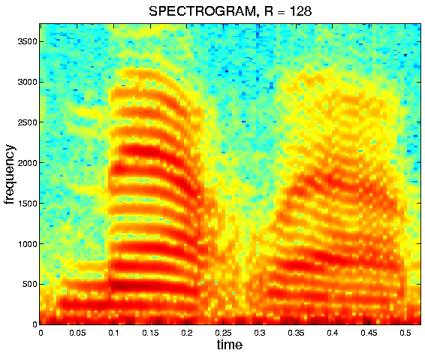
\includegraphics[height=0.40\textwidth]{Wide-band-spectrogram.png}
	\caption{Result of the uncertainty principle: it is not possible, to obtain a high time and frequency resolution at the same time: above are a narrow-band spectrogram (left), wich provides a better frequency resolution and a wide-band spectrogram(right), wich provides a better time resolution of the same signal. Source of pictures: http://cnx.org/content/m10570/latest/} 
\end{figure}\\
If \(g\) is a Gaussian function, then it holds 
	\[\left(\int_{\RR} (x-a)^2|g(x)|^2 \,\mathrm{d}x\right)\left(\int_{\RR}(\omega-b)^2|\FF g(\omega)|^2\,\mathrm{d}\omega\right) = \frac{||g||_2^2}{4\pi}\]
So the Gaussian is the function with minimal uncertainty/  which is equally concentrated in time and frequency. This property of the Gaussian function is used for example in image editing via the Gaussian filter, which is smoothing parts of a picture. (Steht bei Wikipedia, aber eine Quelle, wo der Zusammenhang mathematisch erlaeutert wird, finde ich leider nicht)\\
If \(g\in L^2(\RR^d)\) with \(||g||_2=1\), then, because of the Plancherel equality \(||g||_2=||\FF g||_2\), both \(|g|^2\) and \(|\FF g|^2\) are probability distributions on \(\RR^d\). With \(a=mean(g)\) and \(b=mean(\FF g)\), (\ref{eq:uncertainty}) can be written as
	\[var|g|^2 \cdot var|\FF g|^2 \geq \frac{1}{4\pi},\]
the famous Heisenberg uncertainty principle!\\	
Physically, this result says that position distribution and momentum distribution of a quantum particle cannot be sharply peaked at the same time. Mathematically, one can say that position and momentum are Fourier transforms of one another.\\
In signal analysis, the principle gives a constraint between effective bandwidth and duration of a signal.\\
If we return to our example of audio signals, (\ref{eq:uncertainty}) can be understood in the following way:\\
If the signal \(f\) ist very short, it is not possible to determine the frequencies \(\lambda\) exactly, while on the other hand sound at one exact frequency corresponds to a perfect sine wave with no beginning or ending.

\subsection{Real-Life Applications}
\label{se:real-life}
Sampling is of great importance whenever you need to digitalize and transmit data. 
\subsubsection{Audio signals}
Sound or acoustic noise is produced by vibrating objects, leading to a mechanical wave of pressure through air. This air pressure fluctuations causes the eardrum to oscillate. The auditory ossicle transfer the signal to the cochlea, where parts of the intra cochlea membranes begin to vibrate. The area of the activated membrane depends on the frequency, high frequencies up to 20 kHz are perceived at the base and low frequencies up to 20 Hz at the top of the cochlea. Fine hairs on top of the sensory cells are moved. This motion is converted into an electrochemical impulse of the corresponding auditory nerve. The higher the amplitude of a tone, the higher is the frequency of the action potentials in the nerve.
Hence our auditory organ also applies a short-time Fourier transformation. \\

If we consider now a sound recording as a function $x$, $x$ is obviously compactly supported (there is a strict beginning and end). Consequently the fourier transform $X$ can't be compactly supported ($x$ is not $\omega$-bandlimited). The manner of functioning of our ear allows us to ignore frequencies above 20 kHz and below 20 Hz. Although the reverse fourier transformation $\FF^{-1}(X|_{Q})$ does not coincide with $\FF^{-1}(X)$, for our ear it is of no importance. So by Theorem \ref{th:interpolation}, we can reconstruct such prepared signals with arbitrary precision. 

\begin{figure}[htpb]
\centering
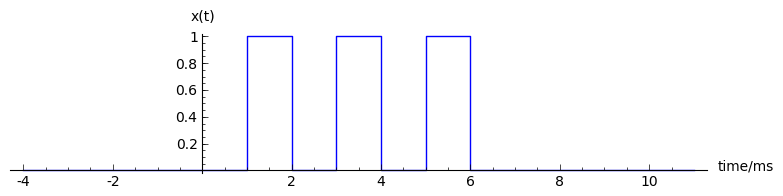
\includegraphics[height=0.3\textwidth]{x(t).png}
\caption{The frequency of $x$ is 2 kHz, thus in our hearable frequency range}
\end{figure}
\begin{figure}[htpb]
\centering
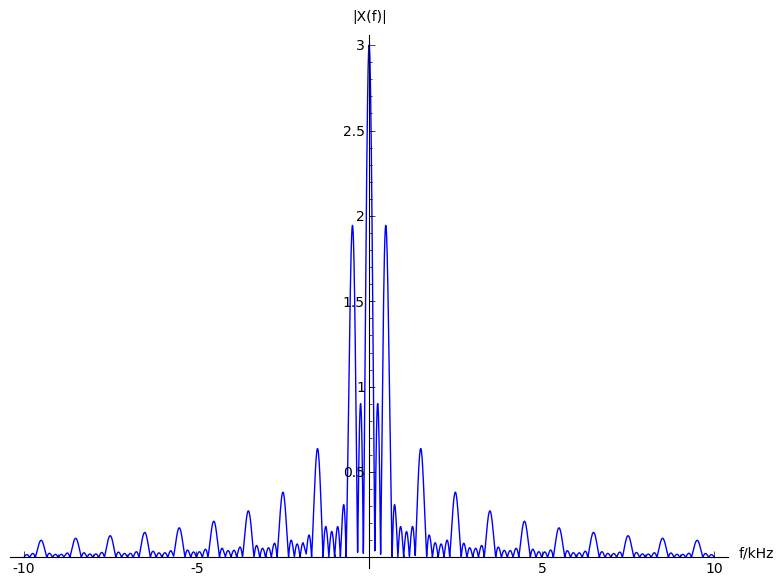
\includegraphics[height=0.646001\textwidth]{X(f).png}
\caption{Here you can see the Fourier transform of \(x\).}

\end{figure}

\newpage
\textbf{Remark}:The cutting of the Frequencies can be realized with a bandpass-filter, a combination of a lowpass- and highpass-filter.A bandlimited function would not be affected by the filtering.\\

\subsubsection*{Pictures and movies}
In the two-dimensional case, one speaks of raster sampling. \\
One application is the television. We reconstruct a moving scene by seeing individual pictures. The rate needed for this is given by the Theorem.\\
Moreover to avoid aliasing (see below), the spectrum of the optical signal must be bounded.(See[3])\\
Also you can use the interpolation formula to reconstruct digitalized pictures or identify small pieces with its place in the whole picture.\\




\subsection*{Dealing with limitations}
As determined above, we have to deal with restrictions in real-life applications.\\
Thus by reconstructing real functions or signals by the Whittaker-Shannon theorem, we have to examine some errors.(see[3])
\begin{itemize}
\item Aliasing:\\
We get an error by sampling a not truly bandlimited function or sampling with a sampling rate below the Nyquist rate (Undersampling). Then the generated spectra would overlap. This is called aliasing. The low frequencies can be regarded, but we lost the high ones. To improve this, you need to sample with a higher rate, if this is technically possible.\\

\item truncation error:\\
Assuming the function is perfect and satisfies all required conditions in the Sampling Theorem, one will have to be content with only a finite number of samples. Let $ f_N(x) $ be the function calculated by Whittaker-Shannon with N samples sampled with the Nyquist rate $ \frac{1}{2\tau_0} $. Like we said above, we can get arbitrary near to the desired function $f(x)$ by increasing N. The remaining so called truncation error $ e_N(t)=\vert f(x)-f_N(x)\vert^2 $ satisfies the inequality \[ e_N(t) \leq N2\tau_0\]\\
Proof see [3]

\item noise:\\
In reality, the signal $x(t) $ we want to sample can be disturbed by random noise $\chi(t)$. The sampled signal is then $ y(t)=x(t)+\chi(t) $. In 1-D, our reconstructed function \[ \tilde{y}(t) = \sum_{k \in \ZZ} y^c(\tau k)  sinc\left(\tau_i^{-1} t_i -k_i\right)=x(t)+\eta(t) \] with $ \eta(t) $ independent of the signal and with mean zero.\\
We can reduce the noise by oversampling or filtering.
\end{itemize}


\nocite{marks02}
\nocite{fornasier03}

\bibliography{literature}
\bibliographystyle{plain}
\end{document}
